%
% SHOW DISENTANGLING: SHAPE
% \begin{figure}[t]\label{fig:shape}
	% \begin{subfigure}{0.5\textwidth}
	% \centering
	% 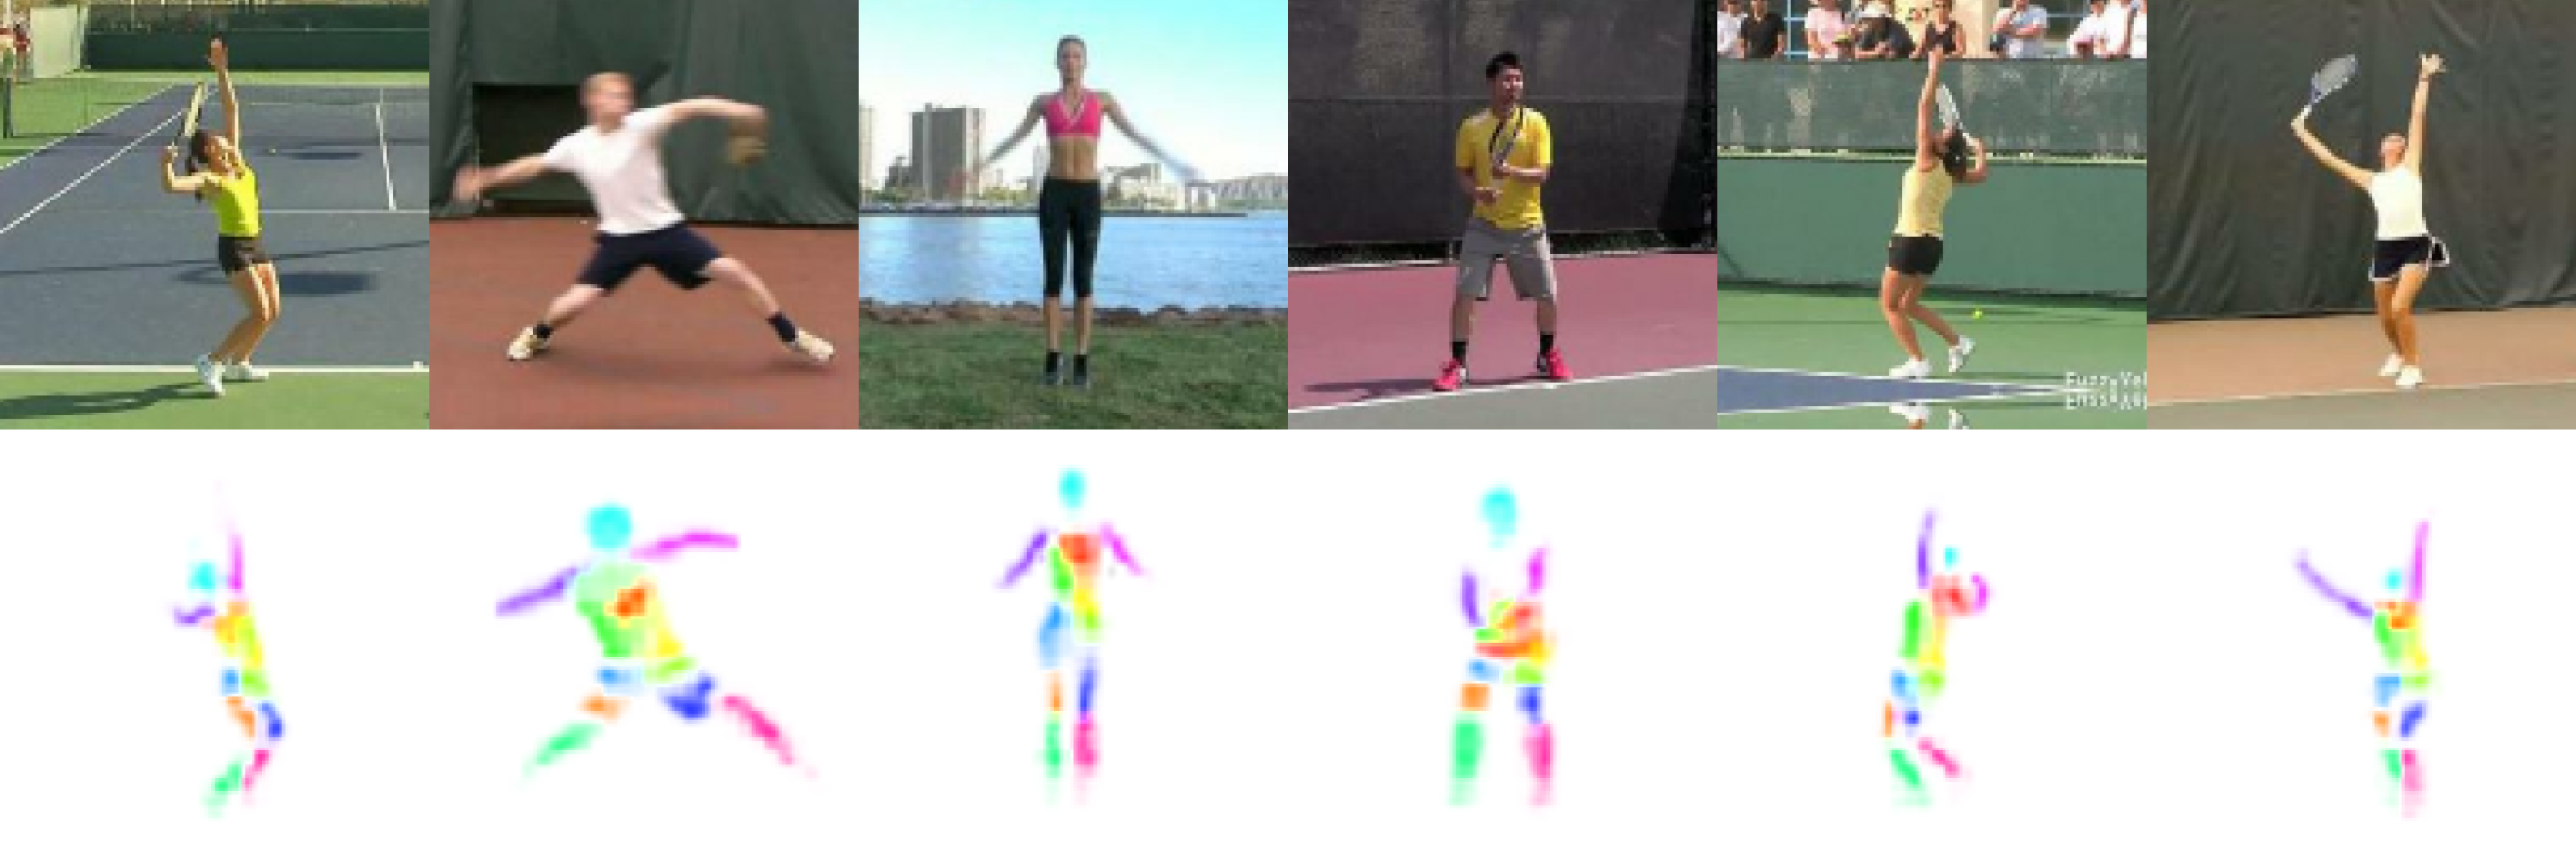
\includegraphics[trim={0cm 0cm 0cm 0cm},clip, width=1.\linewidth]{mat/shape6white}\caption{}
	% \label{fig:shape_penn}
	% \end{subfigure}
	% \begin{subfigure}{0.5\textwidth}
	% \centering
	% 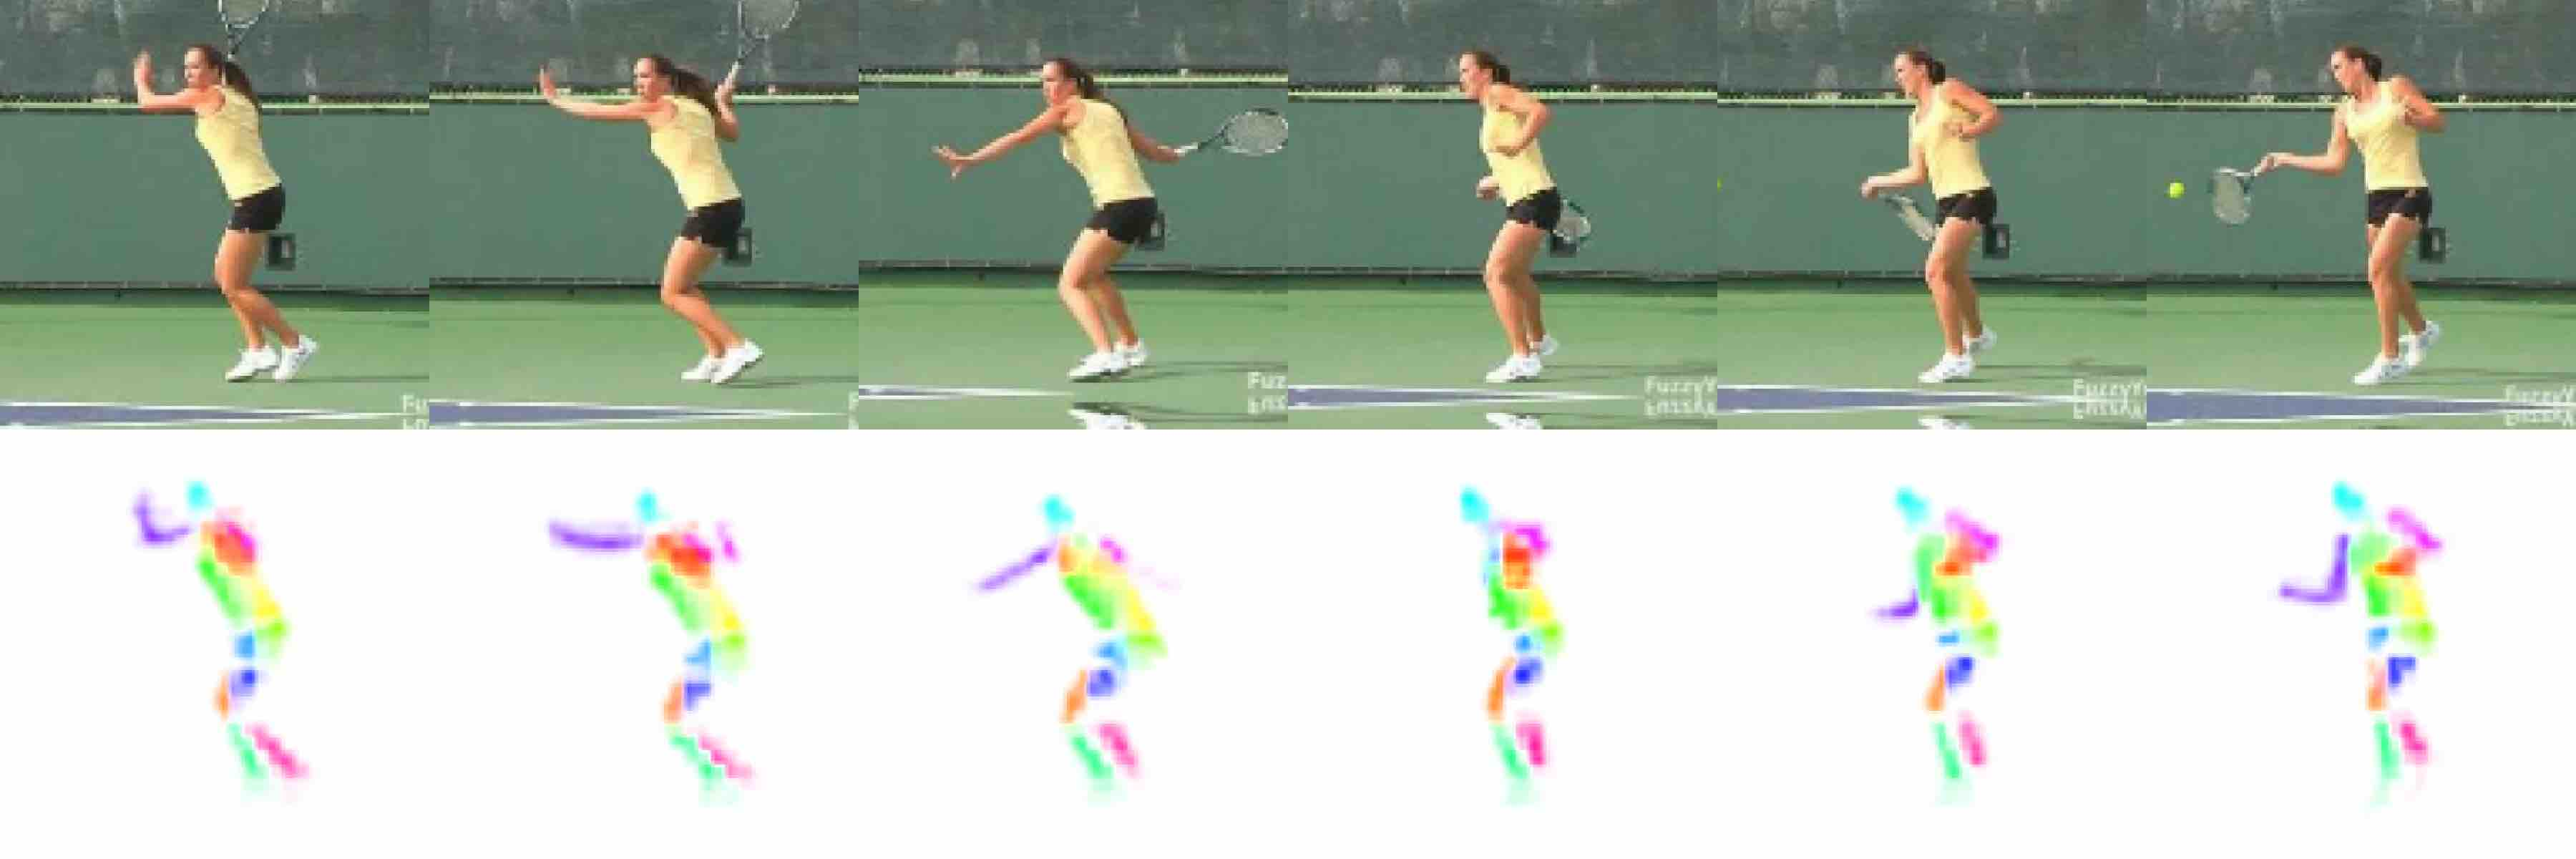
\includegraphics[trim={0cm 0cm 0cm 0cm},clip, width=1.\linewidth]{mat/shape_tennis}\caption{}
	% \label{fig:shape_tennis}
	% \end{subfigure}
	% %\begin{subfigure}{0.5\textwidth}
	% %\centering
	% %\includegraphics[trim={0cm 0cm 0cm 0cm},clip, width=1.\linewidth]{mat/shape_yoga}\caption{}
	% %\label{fig:shape_yoga}
	% %\end{subfigure}
	% \caption{Shape representation on Penn Action. For visualization, all part activation maps are plotted in one image. (a) Different instances, showing intra-class consistency and (b) a time sequence, showing consistency and smoothness under motion.}
% \end{figure}
% POSE APPEARANCE SWAP
\begin{figure}[t]
	\centering
	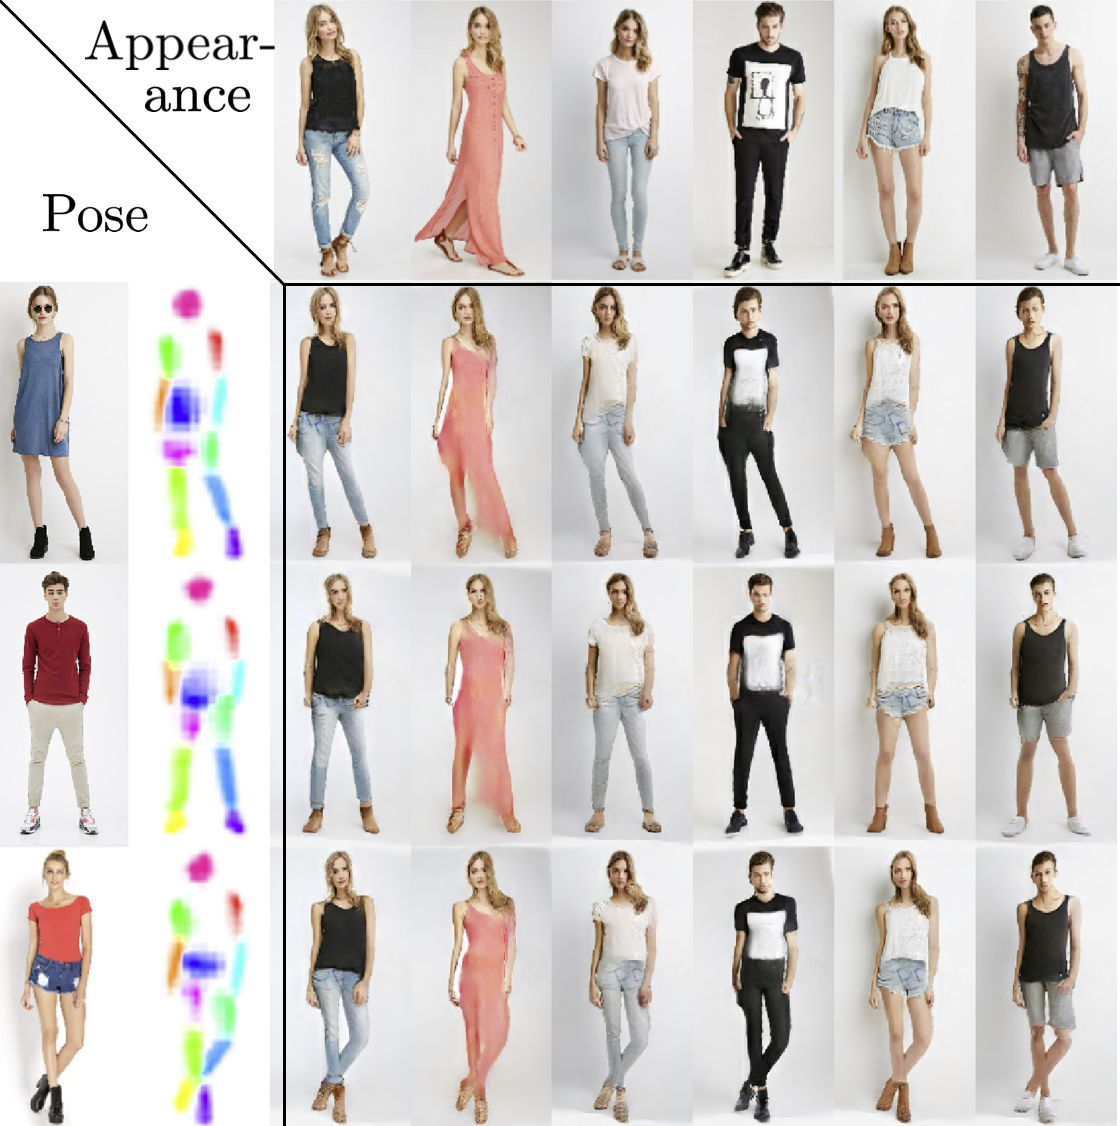
\includegraphics[trim={0cm 0cm 0cm 0cm},clip, width=1.\linewidth]{fig/swappy}
	\caption{Transferring shape and appearance on Deep Fashion. Without annotation the model estimates shape, 2nd column. Target appearance is extracted from images in top row to synthesize images. Note that we trained without image pairs only using synthetic transformations.
	%for training we had no image pairs but only synthetic transformations.
	%without being explicitly trained for this task.
	All images are from test set.}
	\label{fig:allswaps}
\end{figure}
%
